\section{Contexte}
L'association Baleinev organise, depuis plus de 25 ans, le festival de musique “Baleinev Festival” sur le campus de la HEIG-VD et aime se démarquer par son originalité.

En 2014, le festival proposait pour la première fois “Pimp My Wall”, un concept consistant en l'utilisation des fenêtres orientées sur la cour comme écrans géants, affichant du contenu interactif, des animations visuelles et la possibilité de dessiner à distance.

En 2018, le concept a été repris à partir de zéro et a donné naissance à “BeeScreens”, la nouvelle version open source aux technologies modernes. L'ambition du projet est de concevoir un système permettant le développement d'applications interactives diffusées en continu sur Internet (applications, jeux, multi-joueurs, multi-écrans, tout est imaginable). Sa première utilisation a remporté un certain succès lors du Baleinev Festival 2019 !

Baleinev a proposé un premier travail de bachelor en 2019 autour de BeeScreens. Celui-ci a été effectué avec succès et a remporté un prix. Suite à cette bonne expérience, l'association souhaite proposer à nouveau des travaux de bachelor autour de cette thématique.

C'est dans ce contexte-ci qu'est né le projet de ce travail de Bachelor. L'idée est de créer une nouvelle application interactive à projeter sur un sous-ensemble des écrans du festival.

\section{Présentation r/place}
Reddit (\href{https://www.reddit.com}{reddit.com}), sûrement le forum en ligne le plus connu au monde a l'habitude de faire des expériences pour le 1er avril. En 2017, reddit présente pour la première fois leur concept de r/place.

r/place \cite{rplace} offre une toile géante virtuelle permettant à tout le monde de placer un pixel d'une couleur choisie parmi une liste prédéfinie. Chaque utilisateur doit attendre un certain délai (5 minutes) avant de reposer un nouveau pixel, ce qui implique qu'aucun individu ou groupe ne peut nuire trop fortement à l'ensemble de l'oeuvre. Cela oblige une collaboration des utilisateurs afin de réaliser des dessins de qualité.

En 2022, une nouvelle version du r/place est mise en place et plus de 6 millions de joueurs participent à cette édition. La toile est agrandie pour atteindre des dimensions de 2000x2000 pixels est celle-ci se trouve remplie de créations en tout genre réalisées par diverses communautés (voir figure \ref{fig:rplace2022}) pendant plusieurs jours.

\begin{figure}[H]
  \centering
  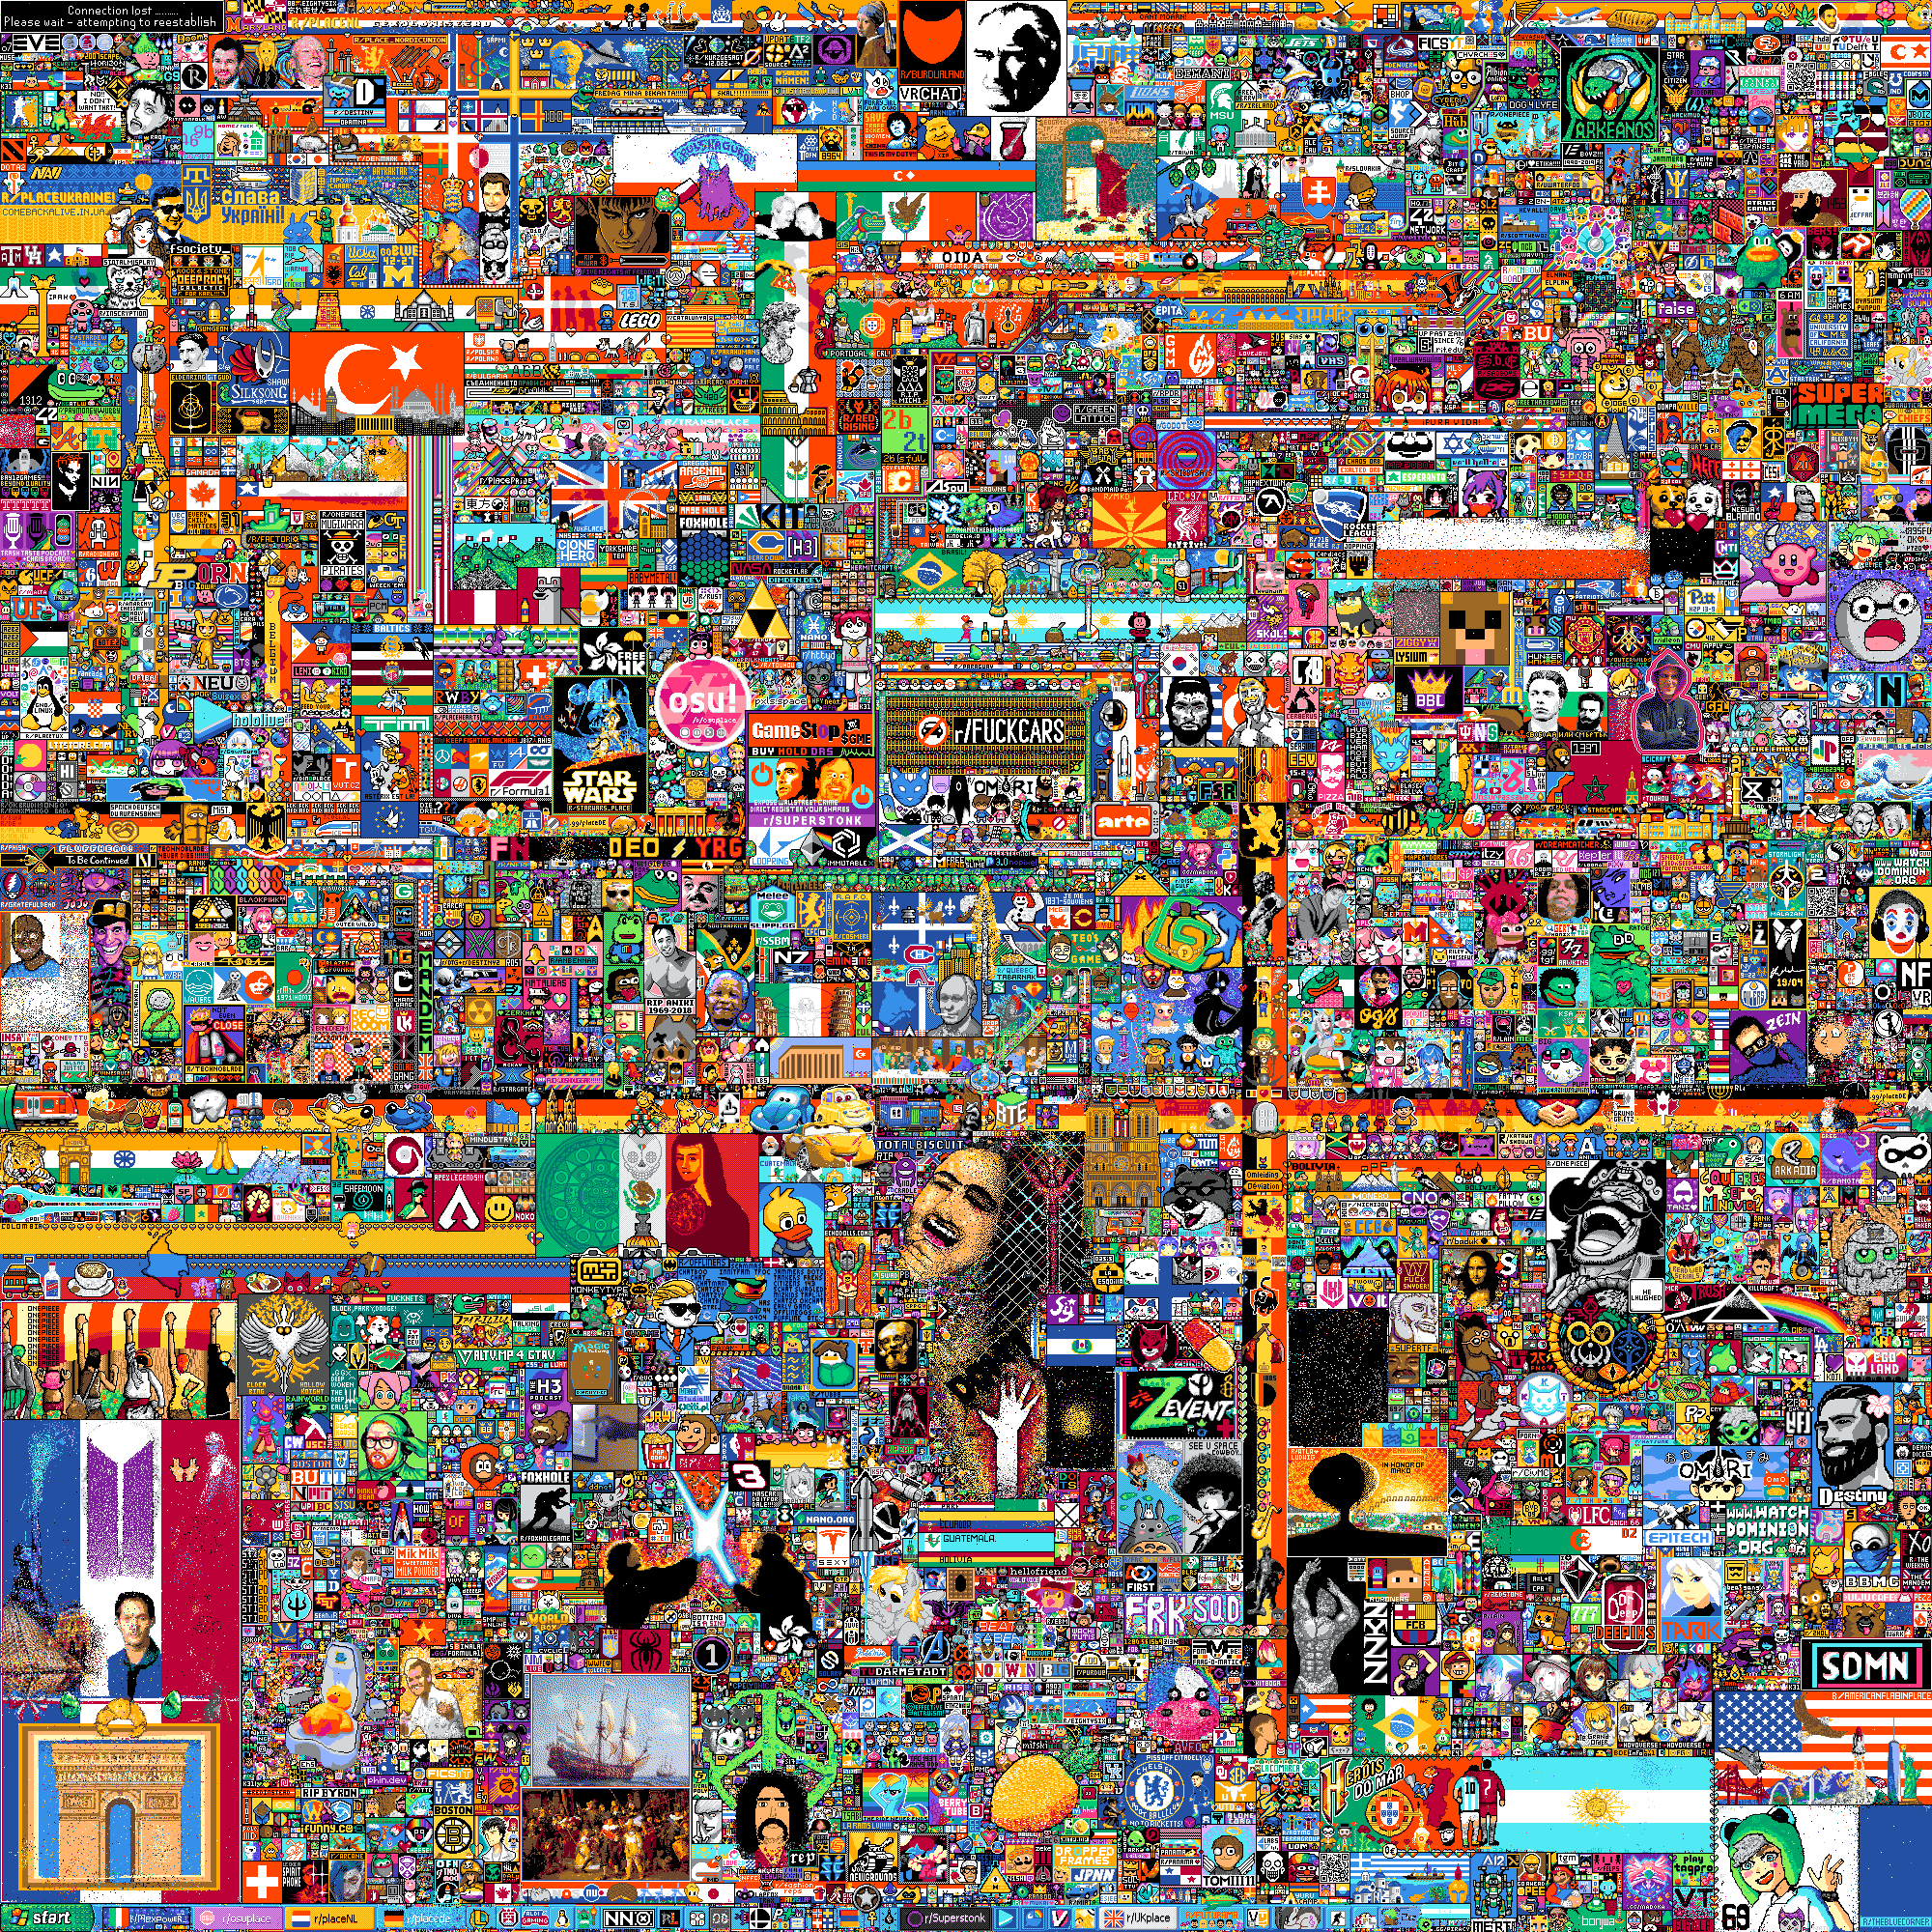
\includegraphics[width=0.8\textwidth]{./assets/figures/rplace.png}
  \caption{Résultat du r/place de 2022}
  \label{fig:rplace2022}
\end{figure}

Les codes sources de ces deux événements ne sont malheureusement pas disponibles. Cependant, les ingénieurs du r/place ont publié des articles détaillant leur architecture et leur implémentation. Ces articles sont disponibles sur le site de reddit \cite{rplace2017, rplace2022}. Ces articles seront utilisés comme référence pour ce travail de bachelor mais l'architecture ainsi que l'implémentation seront complètement différentes. En effet, le but est de créer seul une version open source de r/place. L'envergure du projet ainsi que la taille du public visé sont évidents bien moindres que ceux du r/place original.

\section{Cahier des charges}

\subsection{Présentation}

Le projet principal de ce travail de bachelor consiste en premier lieu à recréer une version Open Source du fameux r/place de Reddit. Cette variante nommée b/place comme référence au festival Baleinev ainsi qu'à BeeScreens.

En plus de reproduire une plateforme dans le genre d'r/place, l'ambition est d'associer si le temps le permet le physique au virtuel. L'idée est de pouvoir proposer aux festivaliers une nouvelle façon de socialiser lors de la soirée. Voici un exemple d'implémentation possible: chaque festivalier aura initialement la possibilité de placer un nombre limité de pixels sur la toile virtuelle géante. Afin d'en avoir davantage, le festivalier devra se rendre à un endroit spécifique appelé la “borne à pixels”. Pour rendre l'expérience plus sociale, l'utilisateur aura l'obligation de scanner le QR Code d'un autre festivalier sur la borne pour recevoir ses précieux pixels.

Pour résumer le travail à effectuer, voici les points importants à retenir:

\begin{itemize}
  \item Développer une application web dans l'idée de r/place.
  \item Assurer l'intégration continue de l'application au sein de l'écosystème BeeScreens.
  \item Assurer la scalabilité de l'application afin de supporter des possibles montées en charges, notamment le soir du festival.
  \item Imaginer et créer un système permettant de lier le virtuel au physique si le temps le permet.
\end{itemize}

\subsection{Objectifs}

Les livrables à réaliser pour ce travail de bachelor sont les suivants:

\begin{itemize}
  \item Un rapport intermédiaire,
  \item Un rapport final,
  \item Un résumé publiable,
  \item Un poster,
  \item L'application web du r/place en elle-même.
\end{itemize}

L'application répond à plusieurs objectifs, catégorisées selon leur importance. Les objectifs \textbf{required} sont nécessaires au bon fonctionnement de l'application. Les \textbf{essential} aident beaucoup à la qualité du projet final et pour finir les \textbf{nice-to-have} améliorent surtout l'expérience utilisateur des usagers ainsi que des administrateurs qui ont la tâche de supprimer les éventuels débordements.

\subsubsection{Objectifs \guillemotleft required\guillemotright}

\begin{itemize}
  \item L'utilisateur arrive sur une page affichant la toile virtuelle au complet.
  \item La toile s'actualise avec les modifications réalisées par les autres utilisateurs.
  \item L'utilisateur peut zoomer ou dé-zoomer sur la toile afin de voir les moindres détails.
  \item L'utilisateur voit facilement le nombre de pixels qu'il a actuellement la possibilité de placer sur la toile.
  \item L'utilisateur peut sélectionner un pixel, choisir une couleur parmi plusieurs proposées et le colorier.
  \item Les dimensions de la toile doivent être configurables par un administrateur.
  \item L'utilisateur dispose d'un moyen de recharger ses pixels à placer une fois ceux-ci écoulés. Il peut par exemple recevoir un nombre de pixels définis après un temps d'attente également choisi.
\end{itemize}

\subsubsection{Objectifs \guillemotleft essential\guillemotright}

\begin{itemize}
  \item Il doit être possible de passer la toile dans un mode “lecture uniquement” par un administrateur pour tous les utilisateurs.
  \item Créer des tests de montée en charge de l'application afin d'assurer un bon fonctionnement lors des festivals notamment.
  \item Afin d'éviter que les utilisateurs puissent recharger la page pour recevoir à nouveau des pixels, trouver un moyen de les identifier.
  \item Les coordonnées du pixel sélectionné par l'utilisateur lui sont affichées ainsi que son niveau de zoom.
  \item Créer des tests unitaires ainsi que des tests d'intégration pour s'assurer de la qualité de l'application.
  \item Un administrateur peut choisir une zone à censurer (recouvrir/suppression de pixels d'une couleur) à partir d'un call API en cas de comportement non désiré.
\end{itemize}

\subsubsection{Objectifs \guillemotleft nice-to-have\guillemotright}

\begin{itemize}
  \item Ajouter une interface utilisateur permettant aux administrateurs de censurer plus facilement une zone de la toile via le dashboard.
  \item Une fois ses pixels épuisés, l'utilisateur peut les recharger via un moyen physique.
  \item Faire en sorte que les couleurs disponibles aux utilisateurs soient facilement customizables par l'administrateur (ex: via le dashboard).
  \item Les administrateurs peuvent interdire la pose de pixels à des utilisateurs ou des régions spécifiques.
  \item Les administrateurs peuvent changer la taille de la toile dynamiquement dans le dashboard.
  \item Afficher à chaque utilisateur le nombre de festivaliers actuellement connectés sur la toile.
  \item Un mode “affichage”, permettant d'afficher régulièrement un QRCode pour rejoindre la toile virtuelle. En plus de ce QRCode, ajouter des éléments sollicitant l'interaction de l'utilisateur à la manière d'un économiseur d'écran (ex: des pixels qui s'animent de façon indépendante). Ce mode s'élèverait automatiquement dès qu'un utilisateur est actif sur l'application.
  \item Ajouter la possibilité de sauvegarder le dessin.
  \item Intégrer la notion de CRDTs (Conflict-free Replicated Data Type), une structure de données permettant d'éviter les conflits notamment dans les systèmes distribués collaboratifs multi utilisateurs.
\end{itemize}

\subsection{Calendrier}

Le projet est séparé en différentes milestones, les dates celles-ci sont adaptées en fonction des événements clés du semestre, comme les délais de rendu ainsi que le festival Baleinev en lui-même.

\subsubsection{Milestone 1 - semaine du 20 au 26 mars}

\begin{enumerate}
  \item Rédaction du cahier des charges
  \item Rédaction de la partie du rapport concernant l'intégration dans l'environnement BeeScreens
\end{enumerate}

\subsubsection{Milestone 2 - semaine du 17 au 23 avril}

\begin{enumerate}
  \item Intégration à l'environnement BeeScreens de l'application b/place
  \item Réalisation d'une première version de l'application afin d'être potentiellement utilisée lors du festival Baleinev de cette année
\end{enumerate}

\subsubsection{Milestone 3 - semaine du 22 au 28 mai}

\begin{enumerate}
  \item Rédaction du rapport intermédiaire
  \item Utilisation d'outils de tests de montées en charges afin d'identifier les problèmes du code actuel
\end{enumerate}

\subsubsection{Milestone 4 - semaine du 12 au 18 juin}

\begin{enumerate}
  \item Optimisation de l'application afin d'améliorer sa scalabilité
  \item Potentiels tests avec les CRDTs (Conflict-free Replicated Data Type)
\end{enumerate}

\subsubsection{Milestone 5 - semaine du 24 au 30 juillet}

\begin{enumerate}
  \item Réalisation des derniers livrables: le résumé publiable ainsi que le poster
  \item Finalisation du rapport
  \item Implémentation de fonctionnalités “nice-to-have”
\end{enumerate}

Le travail se termine le jeudi 27 juillet avec la remise du rapport et des autres livrables indiqués plus haut. La défense du travail aura lieu dans les semaines qui suivent.
